\documentclass{standalone}

\usepackage{tikz, libertinus-otf}
\usetikzlibrary{shapes.multipart, arrows, arrows.meta, positioning, graphs, calc}

\tikzstyle{Argument} = [draw, rectangle, rectangle split, rectangle split parts=2, align=center]

\begin{document} 
    
    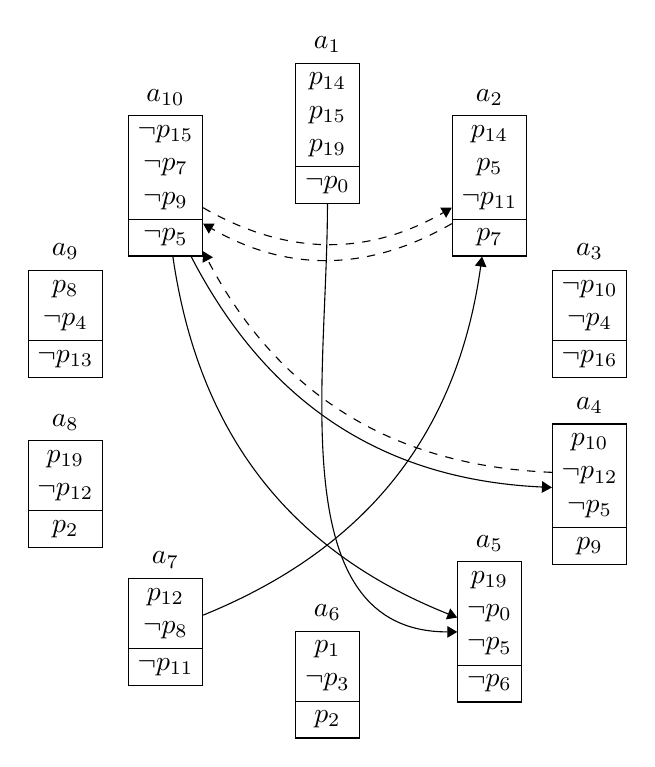
\begin{tikzpicture}
        \begin{scope}[local bounding box=D3]
            \graph [nodes={Argument}, n=10, radius=3.5cm, clockwise]
            {a1/"$p_{14}$\\$p_{15}$\\$p_{19}$\nodepart{two}$\neg p_{0}$"[label=above:$a_1$];
                a2/"$p_{14}$\\$p_{5}$\\$\neg p_{11}$\nodepart{two}$p_{7}$"[label=above:$a_2$];
                a3/"$\neg p_{10}$\\$\neg p_{4}$\nodepart{two}$\neg p_{16}$"[label=above:$a_3$];
                a4/"$p_{10}$\\$\neg p_{12}$\\$\neg p_5$\nodepart{two}$p_{9}$"[label=above:$a_4$];	  
                a5/"$p_{19}$\\$\neg p_{0}$\\$\neg p_5$\nodepart{two}$\neg p_{6}$"[label=above:$a_5$];	  
                a6/"$p_{1}$\\$\neg p_{3}$\nodepart{two}$p_{2}$"[label=above:$a_6$];
                a7/"$p_{12}$\\$\neg p_{8}$\nodepart{two}$\neg p_{11}$"[label=above:$a_7$];
                a8/"$p_{19}$\\$\neg p_{12}$\nodepart{two}$p_{2}$"[label=above:$a_8$];
                a9/"$p_{8}$\\$\neg p_{4}$\nodepart{two}$\neg p_{13}$"[label=above:$a_9$];
                a10/"$\neg p_{15}$\\$\neg p_{7}$\\$\neg p_{9}$\nodepart{two}$\neg p_{5}$"[label=above:$a_{10}$]; 
            }; 
            \draw [-{Triangle[]}] (a1.south) to [out=270,in=180] (a5);
            \draw [dashed, -{Triangle[]}] (a10) to [bend right] (a2);
            \draw [-{Triangle[]}] (a10) to [bend right] (a5);
            \draw [-{Triangle[]}] (a10.290) to [bend right] (a4.170);
            \draw [-{Triangle[]}] (a7) to [bend right] (a2);
            \draw [-{Triangle[]}, dashed] (a2.225) to [bend left] (a10.315);
            \draw [dashed, -{Triangle[]}] (a4.150) to [bend left] (a10.300);
        \end{scope}        
    \end{tikzpicture}
\end{document}